
\begin{tikzpicture}
    \node [examplebox] (box){
        \begin{minipage}{0.475\textwidth}
            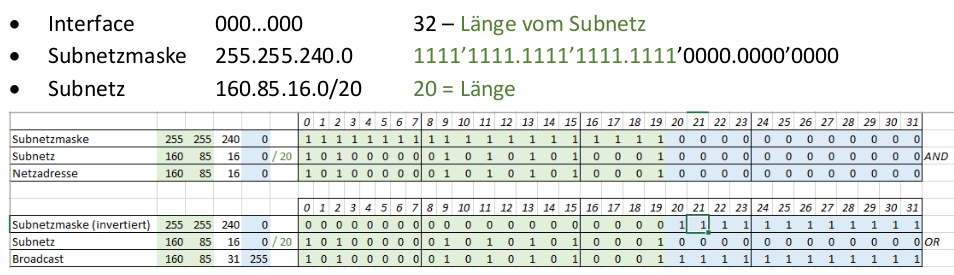
\includegraphics[scale=0.425]{img/ipaddressierung.png}
        \end{minipage}
    };
    \node[exampletitle, right=8pt] at (box.north west) {Addressierung IPv4 Beispiel:};
\end{tikzpicture}



\begin{tikzpicture}
    \node [examplebox] (box){
        \begin{minipage}{0.475\textwidth}
            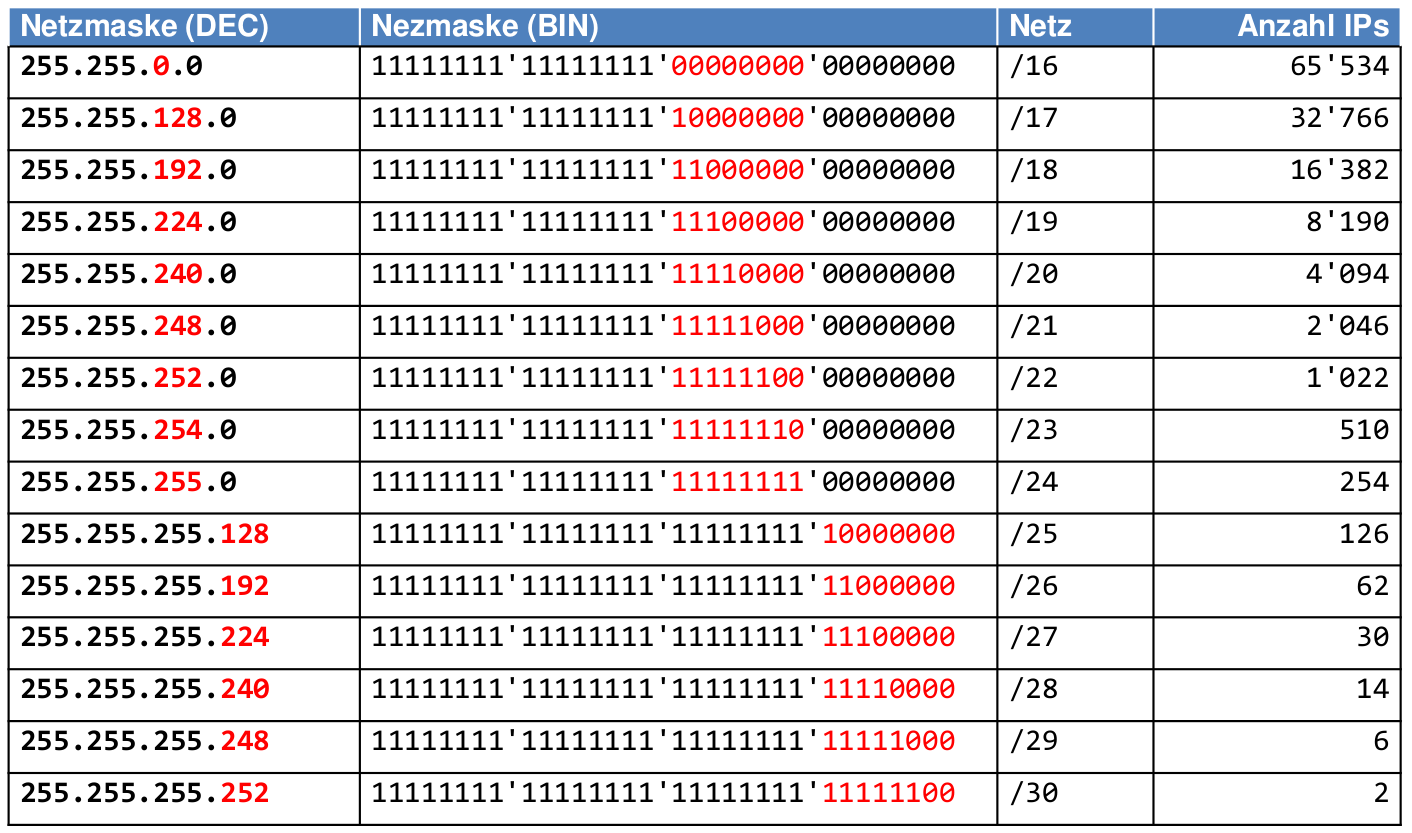
\includegraphics[scale=0.285]{img/subnetzmasken.png}
        \end{minipage}
    };
    \node[exampletitle, right=8pt] at (box.north west) {IP Subnetzmasken};
\end{tikzpicture}




\begin{tikzpicture}
    \node [examplebox] (box){
        \begin{minipage}{0.475\textwidth}
            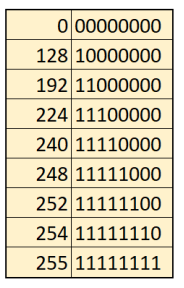
\includegraphics[scale=0.65]{img/binary-subnet.png}

            https://www.itslot.de/2019/02/ipv4-subnetting-berechnen-schritt-fur.html
        \end{minipage}
    };
    \node[exampletitle, right=8pt] at (box.north west) {Subnetze Berechnen};
\end{tikzpicture}


\begin{tikzpicture}
    \node [examplebox] (box){
        \begin{minipage}{0.475\textwidth}
            { Aging-Time: $50$ Sekunden}
            \\
            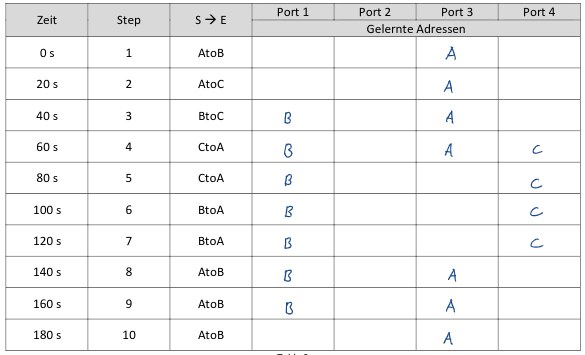
\includegraphics[scale=0.65]{img/filteringdb.png}
        \end{minipage}
    };
    \node[exampletitle, right=8pt] at (box.north west) {Filtering-Database};
\end{tikzpicture}


\begin{tikzpicture}
    \node [examplebox] (box){
        \begin{minipage}{0.475\textwidth}

            177 / 2 \\
            88 / 2 \\
            \unsignedbytecalc{177}

        \end{minipage}
    };
    \node[exampletitle, right=8pt] at (box.north west) {Umrechnung Dezimal zu Binär};
\end{tikzpicture}



\begin{tikzpicture}
    \node [examplebox] (box){
        \begin{minipage}{0.475\textwidth}

            Gegeben ist das Netz 172.30.10.0/25. Dieses Netz soll in drei Subnetze aufgeteilt werden: ein größeres Subnetz 1 für 50 IP-Hosts und zwei kleinere Subnetze 2 und 3 für je 25 IP-Hosts.

            \begin{enumerate}
                \item \textbf{Subnetz 1 für 50 Hosts:}

                      Wir benötigen 6 Bits für die Host-IDs, um mindestens 50 Hosts zu unterstützen (2\^6 - 2 = 62). Das führt zu einer Subnetzmaske von /26 (32 - 6 = 26).

                      \begin{itemize}
                          \item Netzadresse: 172.30.10.0/26
                          \item Broadcastadresse: 172.30.10.63/26
                          \item Anzahl adressierbarer Hosts: 62
                      \end{itemize}

                \item \textbf{Subnetz 2 und 3 für jeweils 25 Hosts:}

                      Wir benötigen 5 Bits für die Host-IDs, um mindestens 25 Hosts zu unterstützen (2\^5 - 2 = 30). Das führt zu einer Subnetzmaske von /27 (32 - 5 = 27).

                      \begin{itemize}
                          \item \textbf{Subnetz 2:}
                                \begin{itemize}
                                    \item Netzadresse: 172.30.10.64/27
                                    \item Broadcastadresse: 172.30.10.95/27
                                    \item Anzahl adressierbarer Hosts: 30
                                \end{itemize}

                          \item \textbf{Subnetz 3:}
                                \begin{itemize}
                                    \item Netzadresse: 172.30.10.96/27
                                    \item Broadcastadresse: 172.30.10.127/27
                                    \item Anzahl adressierbarer Hosts: 30
                                \end{itemize}
                      \end{itemize}
            \end{enumerate}

        \end{minipage}
    };
    \node[exampletitle, right=8pt] at (box.north west) {Subnetting Beispiel 1};
\end{tikzpicture}


\begin{tikzpicture}
    \node [examplebox] (box){
        \begin{minipage}{0.475\textwidth}

            Sie bekommen von Ihrem Internet Service Provider (ISP) ein privates Klasse-C Netz zugeteilt. In Ihrem Haus befinden sich 4 Parteien, welche sich den Internet-Anschluss teilen. Sie geben jeder Partei ein gleich grosses Subnetz, indem sie das Klasse-C Netz 192.168.1.0/24 in 4 Subnetze aufteilen.

            Wir teilen das gegebene Klasse-C Netz 192.168.1.0/24 in vier gleich große Subnetze auf, indem wir zwei zusätzliche Bits für die Subnetz-ID verwenden. Dies führt zu einer neuen Subnetzmaske von /26 und 62 adressierbaren Hosts pro Subnetz ($2^6 - 2 = 62$).

            \begin{enumerate}
                \item \textbf{Subnetz 1:}
                      \begin{itemize}
                          \item Netzadresse: 192.168.1.0/26
                          \item Netzmaske: 255.255.255.192
                          \item Broadcastadresse: 192.168.1.63/26
                          \item Default Gateway: 192.168.1.1 
                          \item Anzahl adressierbarer Hosts: 62
                      \end{itemize}

                \item \textbf{Subnetz 2:}
                      \begin{itemize}
                          \item Netzadresse: 192.168.1.64/26
                          \item Netzmaske: 255.255.255.192
                          \item Broadcastadresse: 192.168.1.127/26
                          \item Default Gateway: 192.168.1.65 
                          \item Anzahl adressierbarer Hosts: 62
                      \end{itemize}

                \item \textbf{Subnetz 3:}
                      \begin{itemize}
                          \item Netzadresse: 192.168.1.128/26
                          \item Netzmaske: 255.255.255.192
                          \item Broadcastadresse: 192.168.1.191/26
                          \item Default Gateway: 192.168.1.129 
                          \item Anzahl adressierbarer Hosts: 62
                      \end{itemize}

                \item \textbf{Subnetz 4:}
                      \begin{itemize}
                          \item Netzadresse: 192.168.1.192/26
                          \item Netzmaske: 255.255.255.192
                          \item Broadcastadresse: 192.168.1.255/26
                          \item Default Gateway: 192.168.1.193 
                          \item Anzahl adressierbarer Hosts: 62
                      \end{itemize}
            \end{enumerate}


        \end{minipage}
    };
    \node[exampletitle, right=8pt] at (box.north west) {Subnetting Beispiel 1};
\end{tikzpicture}



